\documentclass[11pt,]{article}
\usepackage{lmodern}
\usepackage{amssymb,amsmath}
\usepackage{ifxetex,ifluatex}
\usepackage{fixltx2e} % provides \textsubscript
\ifnum 0\ifxetex 1\fi\ifluatex 1\fi=0 % if pdftex
  \usepackage[T1]{fontenc}
  \usepackage[utf8]{inputenc}
\else % if luatex or xelatex
  \ifxetex
    \usepackage{mathspec}
  \else
    \usepackage{fontspec}
  \fi
  \defaultfontfeatures{Ligatures=TeX,Scale=MatchLowercase}
\fi
% use upquote if available, for straight quotes in verbatim environments
\IfFileExists{upquote.sty}{\usepackage{upquote}}{}
% use microtype if available
\IfFileExists{microtype.sty}{%
\usepackage{microtype}
\UseMicrotypeSet[protrusion]{basicmath} % disable protrusion for tt fonts
}{}
\usepackage[margin=1in]{geometry}
\usepackage{hyperref}
\hypersetup{unicode=true,
            pdftitle={Working title: Regression models for Cylindrical data.},
            pdfkeywords={bla vla},
            pdfborder={0 0 0},
            breaklinks=true}
\urlstyle{same}  % don't use monospace font for urls
\usepackage{graphicx,grffile}
\makeatletter
\def\maxwidth{\ifdim\Gin@nat@width>\linewidth\linewidth\else\Gin@nat@width\fi}
\def\maxheight{\ifdim\Gin@nat@height>\textheight\textheight\else\Gin@nat@height\fi}
\makeatother
% Scale images if necessary, so that they will not overflow the page
% margins by default, and it is still possible to overwrite the defaults
% using explicit options in \includegraphics[width, height, ...]{}
\setkeys{Gin}{width=\maxwidth,height=\maxheight,keepaspectratio}
\IfFileExists{parskip.sty}{%
\usepackage{parskip}
}{% else
\setlength{\parindent}{0pt}
\setlength{\parskip}{6pt plus 2pt minus 1pt}
}
\setlength{\emergencystretch}{3em}  % prevent overfull lines
\providecommand{\tightlist}{%
  \setlength{\itemsep}{0pt}\setlength{\parskip}{0pt}}
\setcounter{secnumdepth}{5}
% Redefines (sub)paragraphs to behave more like sections
\ifx\paragraph\undefined\else
\let\oldparagraph\paragraph
\renewcommand{\paragraph}[1]{\oldparagraph{#1}\mbox{}}
\fi
\ifx\subparagraph\undefined\else
\let\oldsubparagraph\subparagraph
\renewcommand{\subparagraph}[1]{\oldsubparagraph{#1}\mbox{}}
\fi

%%% Use protect on footnotes to avoid problems with footnotes in titles
\let\rmarkdownfootnote\footnote%
\def\footnote{\protect\rmarkdownfootnote}

%%% Change title format to be more compact
\usepackage{titling}

% Create subtitle command for use in maketitle
\newcommand{\subtitle}[1]{
  \posttitle{
    \begin{center}\large#1\end{center}
    }
}

\setlength{\droptitle}{-2em}
  \title{Working title: Regression models for Cylindrical data.}
  \pretitle{\vspace{\droptitle}\centering\huge}
  \posttitle{\par}
  \author{Jolien Cremers\footnote{Corresponding author:
  \href{mailto:j.cremers@uu.nl}{\nolinkurl{j.cremers@uu.nl}}} \(^1\),
Helena J.M. Pennings\(^{2,3}\), Christophe Ley \(^{4}\)\\
\(^1\)Department of Methodology and Statistics, Utrecht University\\
\(^2\)TNO\\
\(^3\)Department of Education, Utrecht University\\
\(^4\)Department of Applied Mathematics, Computer Science and
Statistics, Ghent University}
  \preauthor{\centering\large\emph}
  \postauthor{\par}
  \date{}
  \predate{}\postdate{}

\usepackage{booktabs}
\usepackage{longtable}
\usepackage{array}
\usepackage{multirow}
\usepackage[table]{xcolor}
\usepackage{wrapfig}
\usepackage{float}
\usepackage{colortbl}
\usepackage{pdflscape}
\usepackage{tabu}
\usepackage{threeparttable}
\usepackage{threeparttablex}
\usepackage[normalem]{ulem}
\usepackage{makecell}

\usepackage{multirow}
\usepackage{appendix}
\usepackage{color}
\usepackage{hyperref}
\usepackage{subcaption}

\begin{document}
\maketitle
\begin{abstract}
This is the abstract
\end{abstract}

\section{Introduction}\label{Introduction}

Cylindrical data are data that consist of a linear component and a
directional component (a set of angles). In this paper, the directional
component is circular meaning that it consists of a single angle instead
of a set of angles. Figure \ref{} \textcolor{red}{NOG MAKEN} shows the
difference between a circular variable (left) and a linear variable
(right). The most obviuous difference is that on a circular scale the
datapoints 0\(^\circ\) and 360\(^\circ\) are connected and in fact
represent the same number while on a linear scale the two ends,
\(-\infty\) and \(\infty\) are not connected. Cylindrical data occur in
several fields of research, such as for instance in meteorology
(García-Portugués, Crujeiras, \& González-Manteiga, 2013), ecology
(García-Portugués, Barros, Crujeiras, González-Manteiga, \& Pereira,
2014) or marine research (Lagona, Picone, Maruotti, \& Cosoli, 2015).
Several types of data in psychological research are also of a
cylindrical nature. For example, in research on human navigation in the
field of cognitive psychology both distance, a linear variable, and
direction, a circular variable, of movement are of interest (Chrastil \&
Warren, 2017). In eye-tracking research, which is used for investigating
cognitive processes we can also speak of cylindrical data. When
measuring eye-movements we speak of the eye-movements themselves, the
saccades, and fixations, the periods of time between movements when the
eyes are still and looking at one point. Of the saccades both the
direction, a circular variable, and the duration, a linear variable, are
of interest (for a review of eye-tracking research see Rayner (2009)).
Data from circumplex measurement instruments, e.g.~the interpersonal
circumplex as used in personality psychology, are also of a cylindrical
nature (see Section \ref{Example} for a more detailed explanation). In
this paper we will discuss how a correct statistical treatment of such
cylindrical data can lead to new insights. In particular we will show
how cylindrical models pave the way for circular-linear and
linear-circular regression. We will do this for a motivating example
from the field of educational psychology. We will refer to this example
data as the teacher data. In this example, apart from modelling the
relation between the linear and circular component of a cylindrical
variable we would also like to predict the two components from a set of
covariates in a regression model. The teacher data will be further
introduced in Sections \ref{Example} and \ref{DataAnalysis}.

As is the case for circular data, the analysis of cylindrical data
requires special methods. For an overview of methods for circular data
see Mardia \& Jupp (2000) and Jammalamadaka \& Sengupta (2001) and for
modern treatments Ley \& Verdebout (2017). In the literature several
methods have been put forward to model the relation between the linear
and circular component of a cylindrical variable. Some of these are
based on regressing the linear component onto the circular component
using the following type of relation: \[y = \beta_0 + 
\beta_1*\cos(\theta) + \beta_2*\sin(\theta)+ \epsilon,\] where \(y\) is
the linear component and \(\theta\) the circular component (Johnson \&
Wehrly, 1978; Mardia \& Sutton, 1978; Mastrantonio, Maruotti, \&
Jona-Lasinio, 2015). Others model the relation in a different way,
e.g.~by specifying a multivariate model for several linear and circular
variables and modelling their covariance matrix (Mastrantonio, 2018) or
by proposing a joint cylindrical distribution. For example, Abe \& Ley
(2017) introduce a cylindrical distribution based on a Weibull
distribution for the linear component and a sine-skewed von Mises
distribution for the circular component and link these through their
shape and concentration parameters respectively. However, none of the
methods that have been proposed thus far include additional covariates
on which both the circular and linear component are regressed.

Our aim in this paper is to fill this gap in the literature by adapting
four of the existing methods for the analysis of cylindrical data in
such a way that they include a regression of both the linear and
circular component of a cylindrical variable onto a set of covariates.
First however, we will introduce the teacher data in Section
\ref{Example}. In Section \ref{Models} we introduce the four modified
models for cylindrical data that we use to analyze the data from the
motivating example. We also choose a model selection criterion to
compare the models. The teacher data will be analysed in Section
\ref{DataAnalysis}. The paper will be concluded with a discussion in
Section \ref{Discussion}. The Appendix contains technical details.

\section{Teacher data}\label{Example}

The motivating example for this article comes from the field of
educational psychology and was collected for the studies of Pennings et
al. (2017), Claessens (2016) and Want (2015). These studies concern
research on classroom climate. An indicator of classroom climate is the
students' perceptions of their teachers' interpersonal behavior. These
interpersonal perceptions, both in educational psychology as well as in
other areas of psychology, can be measured using circumplex measurement
instruments (see Horowitz \& Strack (2011) for an overview of many such
instruments).

The Questionnaire on Teacher Interaction (QTI) (Wubbels, Brekelmans,
Brok, \& Tartwijk, 2006) is one such circumplex measurement instrument
that can be used to study student perceptions of their teachers'
interpersonal behavior. This instrument contains items that load on two
dimensions: Agency and Communion. Agency refers to the degree of power
or control a teacher exerts in interaction with his/her students.
Communion refers to the degree of friendliness or affiliation a teacher
conveys in interaction with his/her students. The loadings on the two
dimensions of the QTI can be placed in a two-dimensional space formed by
Agency (vertical) and Communion (horizontal), see Figure \ref{QTI}.
Different parts of this space are characterized by different teacher
behavior, e.g. `helpful' or `uncertain'. We call the two-dimensional
space the interpersonal circle (IPC). The idea is that the IPC is ``a
continuous order with no beginning or end'' (Gurtman, 2009, p. 2). We
call such ordering a circumplex ordering and the IPC is therefore often
called the interpersonal circumplex. The ordering also implies that
scores on the IPC could be viewed as a circular variable.

\begin{figure}
\centering
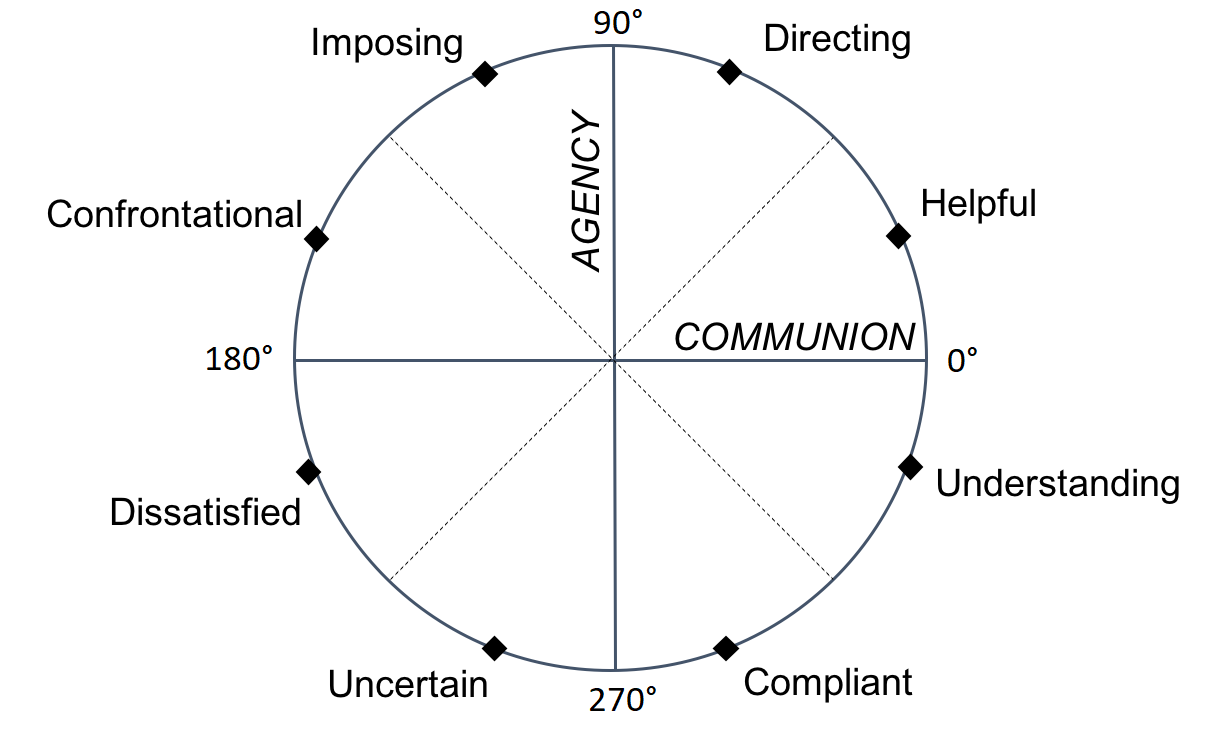
\includegraphics[width = 0.8\textwidth]{IPC-T.png}
\caption{The interpersonal circle for teachers (IPC-T). The words presented in
the circumference of the circle are anchor words to describe the type of
behavior located in each part of the IPC.}
\label{QTI}
\end{figure}

Cremers et al. (2018a) show how data from the IPC can be considered
circular data and analyzed as such using a regression model. The
two-dimension scores Agency and Communion can be converted to a circular
score using the two-argument arctangent function in Equation
\eqref{PredVal}, where \(A\) represents a score on the Agency dimension
and \(C\) represents a score on the Communion dimension. The resulting
circular variable \(\theta\) can then be modeled and for example be
regressed onto covariates in a circular regression model. However, when
two-dimensional data are converted to the circle we lose some
information, namely the length of the two-dimensional vector \((A, C)\),
\emph{i.e.}, its euclidean norm \(\mid\mid (A, C) \mid\mid\). This
length represents the strength of the type of interpersonal behavior a
teacher shows towards his/her students. In a cylindrical model we are
able to incorporate this information, and model a circular variable
\(\theta\) together with a linear variable corresponding to
\(\mid\mid (A, C) \mid\mid\). This will lead to an improved analysis of
data from the IPC. In the next section we will introduce several models
that we can use for a more accurate and more informative regression
analysis on the teacher data. More information on the teacher data will
be given in Section \ref{DataAnalysis}.

\begin{equation}\label{PredVal}
\theta          = \text{atan2}\left(A, \: C\right)  =
\left|{\begin{array}{lcl}
                                                                       \arctan\left(\frac{A}{C}\right) & \text{if}  \quad&C > 0 \\
\arctan\left(\frac{A}{C}\right) + \pi & \text{if}  \quad& C  <  0  \:\: \&\:\: A \geq 0\\
 \arctan\left(\frac{A}{C}\right) - \pi & \text{if}  \quad&C  <  0 \:\:  \&\:\:A  < 0\\
 +\frac{\pi}{2} & \text{if}  \quad& C  =  0  \:\: \&\:\:A > 0\\
 -\frac{\pi}{2} & \text{if}  \quad& C =  0  \:\: \&\:\:A < 0\\
 \text{undefined} & \text{if} \quad& C =  0   \:\: \&\:\:A = 0.
 \end{array}}
\right.
\end{equation}

\section{Four cylindrical regression models}\label{Models}

In this section we will introduce four cylindrical regression models. We
will extend the models from Mastrantonio (2018) and Abe \& Ley (2017) to
contain predictors for the linear and circular outcomes in the
cylindrical model. Additionally we introduce two models where both
variates \(\Theta\) and \(Y\) are predicted by covariates and that model
the relation between the linear and circular outcome as follows
(following Wang, Gelfand, \& Jona-Lasinio (2015) and Mastrantonio et al.
(2015)):

\begin{equation}\label{circlinlink}
y = \gamma_0 + \gamma_{cos}*\cos(\theta)*r + \gamma_{sin}*\sin(\theta)*r + \gamma_1*x_1 + \dots + \gamma_q*x_q +  \epsilon,
\end{equation}

where \(r\) will be introduced in Section \ref{CL-(G)PN}, the error term
\(\epsilon \sim N(0, \sigma)\),
\(\gamma_0, \gamma_{cos}, \gamma_{sin}, \gamma_1, \dots, \gamma_q\) are
the intercept and regression coefficients and \(x_1, \dots, x_q\) are
the \(q\) covariate values. In this model \(Y\) follows a normal
distribution and \(\Theta\) a projected normal (PN) or general projected
normal (GPN) distribution on the circle.

\subsection{The modified CL-PN and modified CL-GPN  models}\label{CL-(G)PN}

In both of these models the relation between the circular variable
\(\Theta \in [0, 2\pi)\) and linear variable
\(Y \in (-\infty, + \infty)\) is specified as in Equation
\ref{circlinlink}. The distribution of \(Y\) conditional on \(\Theta\)
is then given as:

\begin{equation}\label{ycondtheta}
f(y \mid \theta) = \frac{1}{\sqrt{2\pi\sigma^2}}\exp\left[\frac{c^2 + (y - (\gamma_0 + \gamma_1x_1 + \dots + \gamma_qx_q))^{2} - 2c(y - (\gamma_0 + \gamma_1x_1 + \dots + \gamma_qx_q))}{2\sigma^2}\right],
\end{equation}

where
\(c = \begin{bmatrix} r \cos \theta \\ r\sin \theta \end{bmatrix}^t \begin{bmatrix} \gamma_{cos} \\ \gamma_{sin} \end{bmatrix}\),
\(r \geq 0\),
\(\gamma_0, \gamma_{cos}, \gamma_{sin}, \gamma_1, \dots, \gamma_q\) are
the intercept and regression coefficients and \(\sigma^2 \geq 0\) is the
error variance. The linear outcome thus has a normal distribution,
conditional on \(\Theta\).

For the circular outcome we assume either a projected normal (PN) or a
general projected normal (GPN) distribution. These distributions arise
from the radial projection of a distribution defined on the plane onto
the circle. The relation between a bivariate variate \(\boldsymbol{S}\)
in the plane and the circular outcome \(\Theta\) is defined as follows:

\begin{equation}\label{projection}
\boldsymbol{S} = \begin{bmatrix} S^{I} \\ S^{II} \end{bmatrix} = R\boldsymbol{u} = \begin{bmatrix} R \cos \Theta \\  R\sin \Theta \end{bmatrix},
\end{equation}

where \(R = \mid\mid S \mid\mid\), the euclidean norm of the bivariate
vector \(\boldsymbol{S}\). In the PN distribution we assume
\(\boldsymbol{S} \sim N_2(\boldsymbol{\mu}, \boldsymbol{I})\) and in the
GPN we assume
\(\boldsymbol{S} \sim N_2(\boldsymbol{\mu}, \boldsymbol{\Sigma})\) where
\(\boldsymbol{\Sigma} = \begin{bmatrix} \tau^2 + \rho^2 & \rho\\ \rho & 1 \end{bmatrix}\),
\(\rho \in (-\infty, +\infty)\) and \(\tau^2 \geq 0\) (as in
Hernandez-Stumpfhauser, Breidt, \& Woerd (2016)).

Following Nuñez-Antonio, Gutiérrez-Peña, \& Escarela (2011), the joint
density of \(\Theta\) and \(R\) for the PN distribution in a regression
set-up equals:

\begin{equation}\label{pnreg}
f(\theta,r \mid \boldsymbol{\mu}, \boldsymbol{I}) = [2\pi]^{-1} \exp\left[ \frac{-r^2 - \boldsymbol{\mu}^2\boldsymbol{\mu} + 2r\boldsymbol{u}^t\boldsymbol{\mu}}{2}\right],
\end{equation}

In a regression setup the outcome \(\theta_i\) for each individual
\(i = 1, \dots, n\), where \(n\) is the sample size, is generated
independently from Equation (\ref{pnreg}). The mean vector
\(\boldsymbol{\mu}_i \in \mathbb{R}^2\) is defined as
\(\boldsymbol{\mu}_i = \boldsymbol{z}_i\boldsymbol{B}\). The vector
\(\boldsymbol{z}_i\) is a a vector of \(p\) covariate values and
\(\boldsymbol{B} = (\boldsymbol{\beta}^{I}, \boldsymbol{\beta}^{II})\)
contain the regression coefficients. Note however that the dimensions of
\(\boldsymbol{\beta}^{I}\) and \(\boldsymbol{\beta }^{I}\) need not
necessarily be the same and we are thus allowed to have a different set
of predictor variables and vectors \(\boldsymbol{z}_i^I\) and
\(\boldsymbol{z}_i^{II}\) for the two components of
\(\boldsymbol{\mu}_i\).

Following Wang \& Gelfand (2013) and Hernandez-Stumpfhauser et al.
(2016) the joint density of \(r\) and \(\theta\) for the GPN
distribution equals:

\begin{equation}\label{gpnreg}
f(\theta, r \mid \boldsymbol{\mu}, \boldsymbol{\Sigma}) = r(2\pi\tau)^{-1} \exp\left[ -0.5 \sigma^2(r\boldsymbol{u}-\boldsymbol{\mu})^{t}\boldsymbol{\Sigma}^{-1}(r\boldsymbol{u}-\boldsymbol{\mu})\right],
\end{equation}

where
\(\boldsymbol{\Sigma} = \begin{bmatrix} \tau^2 + \rho^2 & \rho\\ \rho & 1 \end{bmatrix}\),
\(\boldsymbol{u}= \begin{bmatrix} \cos \theta \\ \sin \theta \end{bmatrix}\).
In a regression setup the outcome \(\theta_i\) for each individual
\(i = 1, \dots, n\), where \(n\) is the sample size, is generated
independently from Equation (\ref{gpnreg}). The mean vector
\(\boldsymbol{\mu}_i \in \mathbb{R}^2\) is defined as
\(\boldsymbol{\mu}_i = \boldsymbol{z}_i(\boldsymbol{\beta}^{I}, \boldsymbol{\beta}^{II})\).
The vector \(\boldsymbol{z}_i\) is a a vector of \(p\) covariate values
and each \(\boldsymbol{\beta}^{k}\) is a vector with two regression
coefficients, one for each of the two components of
\(\boldsymbol{\mu}_i\). Note that for the CL-GPN model we do need to
have the same predictors for both components of \(\boldsymbol{\mu}_i\).

Both cylindrical models introduced in this section are estimated using
MCMC methods. These methods are based on Nuñez-Antonio et al. (2011),
Wang \& Gelfand (2013) and Hernandez-Stumpfhauser et al. (2016) for the
regression of the circular outcome. A detailed description of the
Bayesian estimation and MCMC samplers can be found in Appendices
\ref{A1} and \ref{A2}.

\subsection{The modified Abe-Ley model}\label{WeiSSVM}

This model is an extension of the cylindrical model introduced by Abe \&
Ley (2017) to the regression context. The density of the model for the
pair of the circular variable \(\theta \in [0, 2\pi)\) and linear
variable \(y\) on the positive real half-line \([0, + \infty)\) is:

\begin{equation}\label{WeiSSVMdensity}
f(\theta, y) = \frac{\alpha(\beta)^\alpha}{2\pi\cosh(\kappa)}
                 (1 +\lambda\sin(\theta - \mu))
                 y^{\alpha-1}
                 \exp[-((\beta y)^{\alpha}(1-\tanh(\kappa)\cos(\theta - \mu)))],
\end{equation}

In a regression setup the outcome vector \((\theta_i, y_i)^t\) for each
individual \(i = 1, \dots, n\), where \(n\) is the sample size, is
generated independently from Equation (\ref{WeiSSVMdensity}). The
parameter \(\alpha > 0\) is a linear shape parameter,
\(\beta_i = \exp(\boldsymbol{x}_i^t\boldsymbol{\nu}) > 0\) is a linear
scale parameter,
\(\mu_i = \eta_0 + 2\tan^{-1}(\boldsymbol{z}_i^t\boldsymbol{\eta}) \in [0, 2\pi)\)
is a circular location parameter, \(\kappa > 0\) is a cicular
concentration parameter and \(\lambda \in [-1, 1]\) is a circular
skewness parameter. The parameter \(\boldsymbol{\nu}\) is a vector of
\(q\) regression coefficients and intercept
\(\nu_j \in (-\infty, +\infty)\) where \(j = 0, \dots, q\), for the
prediction of \(y\). The parameter \(\eta_0 \in [0, 2\pi)\) is the
intercept and \(\boldsymbol{\eta}\), is a vector of \(p\) regression
coefficients \(\eta_j \in (-\infty, +\infty)\), where
\(j = 1, \dots, p\), for the prediction of \(\theta\). The vector
\(\boldsymbol{x}_i\) is a vector of predictor values for the prediction
of \(y\) and \(\boldsymbol{z}_i\) is a vector of predictor values for
the prediction of \(\theta\).

As in Abe \& Ley (2017), the conditional distribution of \(y\) given
\(\theta\) is a Weibull distribution with scale \(\alpha\) and shape
\(\beta(1-\tanh(\kappa)\cos(\theta - \mu))^{1-\alpha}\) and the
conditional distribution of \(\theta\) given \(y\) is a sine skewed von
Mises distribution with location parameter \(\mu\) and concentration
parameter \((\beta y)^\alpha\tanh(\kappa)\).

The log-likelihood for this model equals:

\begin{align}\label{WeiSSVMLikelihood}
l(\alpha, \boldsymbol{\nu}, \lambda, \kappa, \boldsymbol{\eta}) 
   &= n[\ln(\alpha) - \ln(2\pi\cosh(\kappa))] + \alpha \sum^{n}_{i = 1} \ln(\exp(\boldsymbol{x}_i^t\boldsymbol{\nu})) \nonumber\\
   &\:\:\:\:+\sum^{n}_{i = 1} \ln(1 +\lambda\sin(\theta_i - \eta_0 + 2\tan^{-1}(\boldsymbol{z}_i^t\boldsymbol{\eta}))) 
   +(\alpha-1)\sum^{n}_{i = 1} \ln(y_i) \nonumber\\
   &\:\:\:\:-\sum^{n}_{i = 1}( \exp(\boldsymbol{x}_i^t\boldsymbol{\nu})y_i)^{\alpha}(1-\tanh(\kappa)\cos(\theta_i - \eta_0 + 2\tan^{-1}(\boldsymbol{z}_i^t\boldsymbol{\eta})))
\end{align}

We can use numerical optimization (Nelder-Mead) to find solutions for
the maximum likelihood (ML) estimates for the parameters of the model.

\subsection{Modified joint projected and skew normal (GPN-SSN)}\label{CL-GPN_multivariate}

This model is an extension of the cylindrical model introduced by
Mastrantonio (2018) to the regression context. The model contains \(p\)
circular outcomes and \(q\) linear outcomes. The circular outcomes
\(\boldsymbol{\Theta} = (\boldsymbol{\Theta}_1, \dots, \boldsymbol{\Theta}_p)\)
are modeled together by a multivariate GPN distribution and the linear
outcomes
\(\boldsymbol{Y} = (\boldsymbol{Y}_1, \dots, \boldsymbol{Y}_q)\) are
modeled together by a multivariate skew normal distribution (Sahu, Dey,
\& Branco, 2003). Because the GPN distribution is modelled using a
so-called augmented representation (as in (\ref{projection}) and
(\ref{gpnreg})) it is convenient to use a similar tactic for modelling
the multivariate skew normal distribution. As in Mastrantonio (2018) we
use the following representation of the linear outcomes:

\[\boldsymbol{Y} = \boldsymbol{\mu}_y + \boldsymbol{\Lambda}\boldsymbol{D} + \boldsymbol{H},\]
where where \(\boldsymbol{\mu}_y\) is a mean vector for the linear
outcome \(\boldsymbol{Y}\),
\(\boldsymbol{\Lambda} = \text{diag}(\boldsymbol{\lambda})\) is a
\(q \times q\) diagonal matrix with diagonal elements
\(\boldsymbol{\lambda} = \lambda_1, \dots, \lambda_q\) (the parameters
that indicate the skewness of the linear outcomes),
\(\boldsymbol{D} \sim HN_q(\boldsymbol{0}_q, \boldsymbol{I}_q)\), a
q-dimensional half normal distribution (Olmos, Varela, Gómez, \&
Bolfarine, 2012) and
\(\boldsymbol{H} \sim N_q(\boldsymbol{0}_q, \boldsymbol{\Sigma}_y)\).
This means that conditional on the auxiliary data \(\boldsymbol{D}\),
\(\boldsymbol{Y}\) is normally distributed with mean
\(\boldsymbol{\mu}_y + \boldsymbol{\Lambda}\boldsymbol{D}\) and
covariance matrix \(\boldsymbol{\Sigma}_y\). The joint density for
\((\boldsymbol{Y}, \boldsymbol{D})^t\) is defined as follows:

\begin{equation}\label{YDjoint}
f(\boldsymbol{y}, \boldsymbol{d}) = 2^q\phi_q(\boldsymbol{y} \mid \boldsymbol{\mu}_y + \boldsymbol{\Lambda}\boldsymbol{d}, \boldsymbol{\Sigma}_y) \phi_1(\boldsymbol{d} \mid \boldsymbol{0}_q, \boldsymbol{I}_q).
\end{equation}

As in Mastrantonio (2018) dependence between the linear and circular
outcome is created by modelling the augmented representations of
\(\boldsymbol{\Theta}\), and \(\boldsymbol{Y}\) together in a
\(2 \times p + q\) dimensional normal distribution. The joint density of
the model is then represented by:

\begin{equation}\label{YDThetarjoint}
f(\boldsymbol{\theta}, \boldsymbol{r}, \boldsymbol{y}, \boldsymbol{d}) = 2^q\phi_{2p+q}((\boldsymbol{s}, \boldsymbol{y})^t \mid \boldsymbol{\mu} + (\boldsymbol{0}_{2p}, diag(\boldsymbol{\lambda})\boldsymbol{d})^t, \boldsymbol{\Sigma}) \phi_q(\boldsymbol{d} \mid \boldsymbol{0}_q, \boldsymbol{I}_q) \prod_{j = 1}^{p}r_j,
\end{equation}

where the mean vector
\(\boldsymbol{\mu} = (\boldsymbol{\mu}_s, \boldsymbol{\mu}_y)^t\) and
\(\boldsymbol{\Sigma} = \left ( \begin{matrix} \boldsymbol{\Sigma}_s & \boldsymbol{\Sigma}_{sy} \\ \boldsymbol{\Sigma}_{sy^t} & \boldsymbol{\Sigma}_y \\ \end{matrix} \right )\).
The matrix \(\boldsymbol{\Sigma}_s\) is the covariance matrix for the
variances of and covariances between the augmented representations of
the circular outcome and the matrix \(\boldsymbol{\Sigma}_{sy}\)
contains covariances between the augmented representations of the
circular outcome and the linear outcome.

In our regression extension we have \(i = 1, \dots, n\) observations of
\(p\) circular outcomes, \(q\) linear outcomes and \(k\) covariates. The
mean in the density in (\ref{YDThetarjoint}) then becomes
\(\boldsymbol{\mu}_i = \boldsymbol{x}_i\boldsymbol{B}\) where
\(\boldsymbol{B}\) is a \(k \times (2 \times p + q)\) matrix with
regression coeffients. We estimate the model using MCMC methods. A
detailed description of these methods is given in Appendix \ref{A3}.

\subsection{Model fit criterion}\label{Modelfit}

For the four cylindrical models we focus on their out-of-sample
predictive performance to determine the fit of the model. To do so we
split our data in a training and holdout set (10 \(\%\) of the sample).
A proper criterion to compare out-of-sample predictive performance is
the the Predictive Log Scoring Loss (PLSL) (Gneiting \& Raftery, 2007).
The lower the value of this criterion, the better the predictive
performance of the model. Using ML estimates this criterion can be
computed as follows:

\begin{equation}\label{PLSLML}
PLSL = -2 \sum_{i = 1}^{M}\log l(x_i \mid \hat{\boldsymbol{\vartheta}}),
\end{equation}

where \(l\) is the model likelihood, \(M\) is the sample size of the
holdout set, \(x_i\) is the \(i^{th}\) datapoint from the holdout set
and \(\hat{\boldsymbol{\vartheta}}\) are the ML estimates of the model
parameters. Using posterior samples the criterion is similar to the log
pointwise predictive density (lppd) as outlined in Gelman et al. (2014)
and can be computed as:

\begin{equation}\label{PLSLBayes}
PLSL = -2 \frac{1}{B} \sum_{j = 1}^{B}\sum_{i = 1}^{M} \log l(x_i \mid \boldsymbol{\vartheta}^{(j)}),
\end{equation}

where \(B\) is the amount of posterior samples and
\(\boldsymbol{\vartheta}^{(j)}\) are the posterior estimates of the
model parameters for the \(j^{th}\) iteration. Note that although we fit
the CL-PN, CL-GPN and joint GPN-SSN models using Bayesian statistics, we
do not take prior information (only the likelihood) into account when
assessing model fit. According to Gelman et al. (2014) this is not
necessary since we are assessing the fit of a model to data only
\textcolor{red}{AFMAKEN!}. For each of the cylindrical models we can
then compute a PLSL for the circular and linear outcome by using the
conditional log-likelihoods of the respective outcome.

\section{Data Analysis}\label{DataAnalysis}

In this section we will analyze the teacher dataset with the help of the
four cylindrical models introduced in Section \ref{Models}. We will
however first give a more detailed description of the dataset.

\subsection{Data description}\label{DataDescriptives}

The teacher data was collected between 2010 and 2015 and contains
several repeated measures on the IPC of 161 teachers gathered for the
studies of Want (2015), Claessens (2016) and Pennings et al. (2017). The
measurements were obtained using the QTI and taken in different years
and in different classes. For this paper we only consider one
measurement, namely the one for the first measurement occasion (2010)
and the one for the largest class if data for multiple classes were
available. In addition to a variable \texttt{IPC} containing the
circular outcome and the `length' of the IPC, the linear outcome, a
teachers' self-efficacy (\verb|SE|) will be used as covariate in the
analysis. After the removal of missing cases we end up with a sample of
148 teachers Table \ref{Tableteacherdescriptives} shows descriptives for
the dataset.

\begin{table}
\centering
\caption{Descriptives for the teacher dataset} 
\begin{tabular}{lrrrl}
  \noalign{\smallskip}\hline\noalign{\smallskip}
Variable & mean/$\bar{\theta}$ & sd/$\hat{\rho}$ & Range & Type \\ \hline\noalign{\smallskip}
IPC &33.23$^\circ$& 0.76 & - & Circular\\
length IPC & 0.43 & 0.15 & 0.08 - 0.80 & Linear\\
SE & 4.72 & 0.87 & 2 - 6.5 & Linear\\
   \hline
\end{tabular}
\label{Tableteacherdescriptives}
\caption*{Note that $\hat{\rho}$ is an sample estimate for the circular concentration where a value of 0 means that the data is not concentrated at all, i.e. spread over the entire circle, and a value of 1 means that all data is concentrated at a single point on the circle. }
\end{table}

\subsection{Models}\label{DataModels}

The regression equations for the linear and the circular outcome of the
four cylindrical models fit to the teacher dataset are as follows:

\begin{itemize}
\item For the modified CL-PN and CL-GPN models:

$\hat{\boldsymbol{\mu}}_{i} = \begin{pmatrix}
  \mu_{i}^{I}  \\
\mu_{i}^{II}
 \end{pmatrix}=\begin{pmatrix}
  \beta_0^{I} + \beta_1^{I}\text{SE}_i  \\
  \beta_0^{II} + \beta_1^{II}\text{SE}_i
 \end{pmatrix},$

$\hat{y}_i = \gamma_0 + \gamma_{cos}\cos\theta_ir_i + \gamma_{sin}\sin\theta_ir_i + \gamma_1\text{SE}_i.$

\item For the modified Abe-Ley model:

$\hat{\mu}_{i} = \eta_0 + 2 * \tan^{-1}(\eta_1\text{SE}_i),$

$\hat{\beta}_{i} = \exp(\nu_0 + \nu_1\text{SE}_i).$

\item For the modified joint projected and skew normal model:

$\hat{\boldsymbol{\mu}}_{i} = \boldsymbol{\beta}_0 + \boldsymbol{\beta}_1\text{SE}_i$, where $\boldsymbol{\mu}_i = (\boldsymbol{\mu}_{s_i}, \boldsymbol{\mu}_{y_i})^t$, $\boldsymbol{\beta}_0 = (\beta_{0_s^{I}}, \beta_{0_s^{II}},\beta_{0_y})$ and $\boldsymbol{\beta}_1 = (\beta_{1_s^{I}}, \beta_{1_s^{II}},\beta_{1_y})$.
\end{itemize}

The variable \verb|SE| is thus used as a predictor for the linear and
circular outcomes in all four cylindrical models. We will use the
loglikelihoods of the following conditional densities
\textcolor{red}{CHRISTOPHE, MAG HIER WEL $\sim$ GEBRUIKT WORDEN?}for the
computation of the PLSL criterion to evaluate the model fit:

\begin{itemize}
\item for the modified CL-PN model:

$y_i \mid \mu_i, \sigma^2 \sim N(\mu_i, \sigma^2)$, where $\mu_i = \hat{y}_i$ and for $\theta_i$ we use Equation (\ref{pnreg}).

\item for the modified CL-GPN model:

$y_i \mid \mu_i, \sigma^2 \sim N(\mu_i, \sigma^2)$, where $\mu_i = \hat{y}_i$ and for $\theta_i$ we use Equation (\ref{gpnreg}).

\item for the modified Abe-Ley model:

$y_i \mid \boldsymbol{\theta}_i, \beta_i, \mu_i, \kappa, \alpha \sim W\left(\beta_i(1-\tanh(\kappa)\cos(\theta_i - \mu_i))^{1/\alpha}, \alpha\right)$, a Weibull distribution.

$\theta_i \mid y_i, \beta_i, \mu_i, \kappa, \alpha \lambda \sim SSVM\left(\mu_i, (\beta_iy_i)^{\alpha}(\tanh{\kappa})\right)$, a sine-skewed von Mises distribution.

\item for the modified joint projected and skew normal model:

$y_i \mid \boldsymbol{\mu}_i, \boldsymbol{\Sigma}, \boldsymbol{\theta}_i, r_i \sim SSN(\mu_{i_y} + \lambda d_i + \boldsymbol{\Sigma}_{sy}^t\boldsymbol{\Sigma}_w^{-1}(\boldsymbol{s}_i - \boldsymbol{\mu}_{i_s}), \boldsymbol{\Sigma}_y + \boldsymbol{\Sigma}_{sy}^t\boldsymbol{\Sigma}_s\boldsymbol{\Sigma}_{sy}),$

$\theta_i \mid \boldsymbol{\mu}_i, \boldsymbol{\Sigma}, y_i, d_i \sim GPN(\boldsymbol{\mu}_{i_s} + \boldsymbol{\Sigma}_{sy}\boldsymbol{\Sigma}_y^{-1} (y_i - \mu_{i_y} - \lambda d_i), \boldsymbol{\Sigma}_s + \boldsymbol{\Sigma}_{sy}\boldsymbol{\Sigma}_y^{-1}\boldsymbol{\Sigma}_{sy}^t)$

where $SSN$ is the skew normal distribution.

\end{itemize}

\subsection{Results \& Analysis}\label{DataResults}

Before analysis there were a couple of settings that we had to specify
for the cylindrical models. Starting values for the WeiSSVM model were
the following
\(\eta_0 = 0.5, \eta_1 = 0.5, \nu_0 = 0.5, \nu_1 = 0.5, \kappa = 0.5, \alpha = 0.5, \lambda = 0\).
The initial amount of iterations for the three MCMC samplers was set to
2000. After we checked convergence via traceplots we concluded that some
of the parameters of the multivariate GPN model did not converge.
Therefore we set the amount of iterations of the MCMC models to 20,000
and subtracted a burn-in of 5000. With this specification the MCMC
chains for all parameters converge. Note that we choose the same amount
of iterations for all three Bayesian cylindrical models to make their
comparison via the PLSL as fair as possible. Lastly, the predictor
\verb|SE| was centered before inclusion in the analysis.

\begin{table}

\caption{\label{tab:estCLGPN}Results for the modified CL-PN and CL-GPN model}
\centering
\begin{tabular}[t]{lrrrrrr}
\toprule
\multicolumn{1}{c}{Parameter} & \multicolumn{3}{c}{CL-PN} & \multicolumn{3}{c}{CL-GPN} \\
\cmidrule(l{2pt}r{2pt}){1-1} \cmidrule(l{2pt}r{2pt}){2-4} \cmidrule(l{2pt}r{2pt}){5-7}
  & Mode & HPD LB & HPD UB & Mode & HPD LB & HPD UB\\
\midrule
$\beta_0^{I}$ & 1.63 & 1.36 & 1.87 & 2.15 & 1.64 & 2.59\\
$\beta_0^{I}$ & 0.52 & 0.23 & 0.80 & 0.65 & 0.14 & 1.06\\
$\beta_0^{II}$ & 1.00 & 0.80 & 1.23 & 1.24 & 0.98 & 1.51\\
$\beta_1^{II}$ & 0.39 & 0.16 & 0.64 & 0.46 & 0.18 & 0.72\\
$\gamma_0$ & 0.35 & 0.29 & 0.41 & 0.35 & 0.30 & 0.40\\
\addlinespace
$\gamma_{cos}$ & 0.05 & 0.02 & 0.07 & 0.04 & 0.02 & 0.06\\
$\gamma_{sin}$ & -0.01 & -0.04 & 0.03 & -0.01 & -0.04 & 0.03\\
$\gamma_1$ & 0.03 & -0.01 & 0.06 & 0.03 & -0.01 & 0.06\\
$\sigma$ & 0.14 & 0.13 & 0.16 & 0.14 & 0.12 & 0.16\\
$\sum_{1,1}$ & NA & NA & NA & 2.67 & 1.77 & 4.12\\
\addlinespace
$\sum_{1,2}$ & NA & NA & NA & 0.81 & 0.53 & 1.07\\
$\sum_{2,2}$ & NA & NA & NA & 1.00 & 1.00 & 1.00\\
\bottomrule
\end{tabular}
\end{table}

\begin{table}

\caption{\label{tab:estSL}Results for the modified Abe-Ley model}
\centering
\begin{tabular}[t]{lr}
\toprule
\multicolumn{1}{c}{Parameter} & \multicolumn{1}{c}{ML-estimate} \\
\cmidrule(l{2pt}r{2pt}){1-1} \cmidrule(l{2pt}r{2pt}){2-2}
$\eta_0$ & 0.37\\
$\eta_1$ & -0.01\\
$\nu_0$ & 1.19\\
$\nu_1$ & 0.00\\
$\alpha$ & 3.82\\
\addlinespace
$\kappa$ & 1.57\\
$\lambda$ & 0.66\\
\bottomrule
\end{tabular}
\end{table}

\begin{table}

\caption{\label{tab:estCLMGPN}Results for the modified joint projected and skew normal model}
\centering
\begin{tabular}[t]{lrrrrrr}
\toprule
\multicolumn{1}{c}{Parameter} & \multicolumn{3}{c}{Unconstrained} & \multicolumn{3}{c}{Constrained} \\
\cmidrule(l{2pt}r{2pt}){1-1} \cmidrule(l{2pt}r{2pt}){2-4} \cmidrule(l{2pt}r{2pt}){5-7}
  & Mode & HPD LB & HPD UB & Mode & HPD LB & HPD UB\\
\midrule
$\beta_{0_s^{I}}$ & 0.30 & 0.26 & 0.34 & 1.94 & 1.63 & 2.33\\
$\beta_{0_s^{II}}$ & 0.19 & 0.16 & 0.21 & 1.20 & 0.98 & 1.43\\
$\beta_{0_y}$ & 0.33 & 0.30 & 0.37 & 0.33 & 0.30 & 0.37\\
$\beta_{1_s^{I}}$ & 0.07 & 0.03 & 0.12 & 0.50 & 0.16 & 0.79\\
$\beta_{0_s^{II}}$ & 0.04 & 0.01 & 0.08 & 0.27 & 0.09 & 0.50\\
\addlinespace
$\beta_{1_y}$ & 0.07 & 0.04 & 0.12 & 0.07 & 0.04 & 0.12\\
$\sum_{s_{1,1}}$ & 0.05 & 0.04 & 0.07 & 2.16 & 1.51 & 2.99\\
$\sum_{s_{2,2}}$ & 0.02 & 0.02 & 0.03 & 1.00 & 1.00 & 1.00\\
$\sum_{y_{3,3}}$ & 0.03 & 0.02 & 0.05 & 0.03 & 0.02 & 0.05\\
$\sum_{s_{1,2}}$ & 0.00 & 0.00 & 0.01 & 0.19 & -0.06 & 0.46\\
\addlinespace
$\sum_{sy_{1,3}}$ & 0.04 & 0.03 & 0.05 & 0.24 & 0.18 & 0.33\\
$\sum_{sy_{2,3}}$ & 0.01 & 0.01 & 0.02 & 0.10 & 0.06 & 0.13\\
$\lambda$ & 0.14 & 0.13 & 0.17 & 0.14 & 0.13 & 0.17\\
\bottomrule
\end{tabular}
\end{table}

Tables 2, 3 and 4 show results from the four models that were fit to the
teacher dataset. There are several parameters that we can compare
between these results. Firstly, we have the estimated mean of the
circular outcome. In Table 5 we see the posterior (predictive)
distributions for the estimated circular means of the CL-PN, CL-GPN and
joint GPN-SSN model. For the CL-PN model we can actually also compute
this means from the estimates in Table 2 as follows:
\(\mu_{circ} = atan2(\beta_0^{II}, \beta_0^{I})\). This leads to an
estimate of 31.53\(^\circ\). The estimates for the CL-PN, CL-GPN and
joint GPN-SSN model are about equal and correspond quite well to the
actual data mean of 33.23\(^\circ\) in Table
\ref{Tableteacherdescriptives}. The estimate from the Abe-Ley model
which is 0.37 radians or 21.20\(^\circ\) is different. This difference
could be caused by the fact that the densities for the circular ouctome,
projected normal or sine-skewed von Mises, differ between the models.

\begin{table}

\caption{\label{tab:means}Posterior estimates for the circular mean in the CL-PN, CL-GPN and joint GPN-SSN models}
\centering
\begin{tabular}[t]{lr}
\toprule
  & Mean (degrees)\\
\midrule
Cl-PN & 31.98\\
CL-GPN & 32.98\\
GPN-SSN & 34.50\\
\bottomrule
\multicolumn{2}{l}{\textsuperscript{a} Note that these means}\\
\multicolumn{2}{l}{are based on the}\\
\multicolumn{2}{l}{posterior predictive}\\
\multicolumn{2}{l}{distribution for the}\\
\multicolumn{2}{l}{intercepts following}\\
\multicolumn{2}{l}{(Wang \& Gelfand,}\\
\multicolumn{2}{l}{2013).}\\
\end{tabular}
\end{table}

We can also compare the effect of \verb|SE| on the circular outcome. For
the CL-PN model and Abe-Ley models we can get estimates of a circular
regression coefficient of this effect. For the Abe-Ley model this
estimate is the parameter \(\nu_1 = -0.01\). This means that for each
unit increate in self-efficacy, at the inflection point of the circular
regression line, the score of the teacher on the IPC decreases with
\(0.01*(180/\pi) = 0.57^\circ\). For the CL-PN model we can use methods
from Cremers et al. (2018b). The estimated posterior mode of \(b_c\), a
parameter that is comparable to \(\nu_1\) in the Abe-Ley model, equals
\(1.13\) and its 95\% HPD interval is \((-26.55; 25.46)\). This means
that for each unit increate in self-efficacy, at the inflection point of
the circular regression line, the score of the teacher on the IPC
increases with \(1.13*(180/\pi) = 74.74^\circ\). Values of \(b_c\) and
\(\nu_1\) are quite different even though they should represent the same
effect. However, the slope at the inflection point, which \(b_c\) and
\(\nu_1\) describe is not necessarily representative of the effect of
\verb|SE| in the data range. In Figure \ref{} we see that the inflection
point (square) for the CL-PN model lies just ouside of the data range
and that for the Abe-Ley model even further (outside the x-axis range).
The slope of both regression lines in the data range is much more alike
(even though one is positive and the other negative). The slope at the
mean Self-efficicay, which has a value of 0 because it was centered,
\(SAM\) is estimated at \(0.02 (-0.09; 0.15)\) The \(SAM\) can be
interpreted as the amount of change on the circle for a unit increase at
the mean of the predictor variable. However, for the CL-PN model the
95\% HPD interval of \(SAM\) for the effect of \verb|SE| includes 0
meaning that the value is not different from 0. For the Abe-Ley model
standard errors of the parameters are not known so we cannot formally
test whether \(\nu_1\) differs from 0. Neither is there a known way of
computing the effect at predictor values other than the one of the
inflection point.

For the CL-GPN and multivariate CL-GPN models we cannot compute circular
regression coefficients. Instead, we will compute posterior predictive
distributions for the predicted circular outcome of individuals scoring
1 unit above and 1 unit below the average self-efficacy.

\begin{figure}
\centering
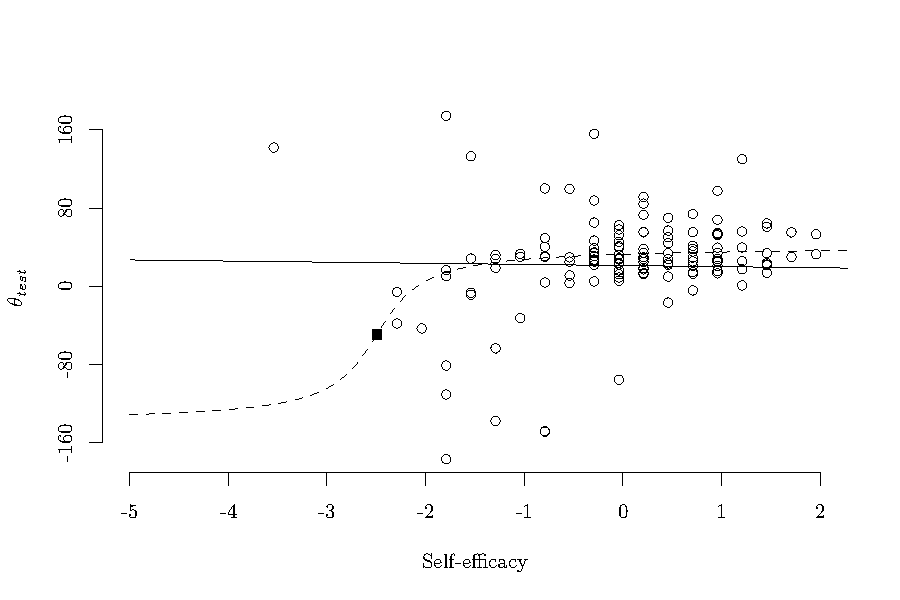
\includegraphics[width = 0.8\textwidth]{regline.pdf}
\caption{Plot showing circular regresion lines as predicted by the Abe-Ley (solid line) and CL-PN model (dashed line).}
\label{regline}
\end{figure}

Next, we compare the intercepts and regression coefficients for the
linear outcome.

\begin{itemize}
\item How to interpret weibull regression for Abe-Ley model?
\item Comment on different distributions for linear and circular outcome ($\lambda$ in multivariate CL-GPN), integrate with model fit does this correspond. 
\item Comment on different estimation methods, in CL-PN and CL-GPN the regression of $\theta$ is independent of $y$ but not vice-versa. In the Abe-Ley and Multivariate method dependence between $\theta$ and $y$ is modelled both ways. 
\end{itemize}

\subsubsection{Model fit}

\begin{table}

\caption{\label{tab:ModelFit}PLSL criteria for the circular and linear outcome in the four cylindrical models}
\centering
\begin{tabular}[t]{lrrrr}
\toprule
  & CL-PN & CL-GPN & Abe-Ley & Joint GPN-SSN\\
\midrule
circular & 86.15 & 52.88 & 58.53 & 103.83\\
linear & -20.17 & -20.32 & 51.83 & 11.98\\
\bottomrule
\end{tabular}
\end{table}

\begin{figure}
\centering
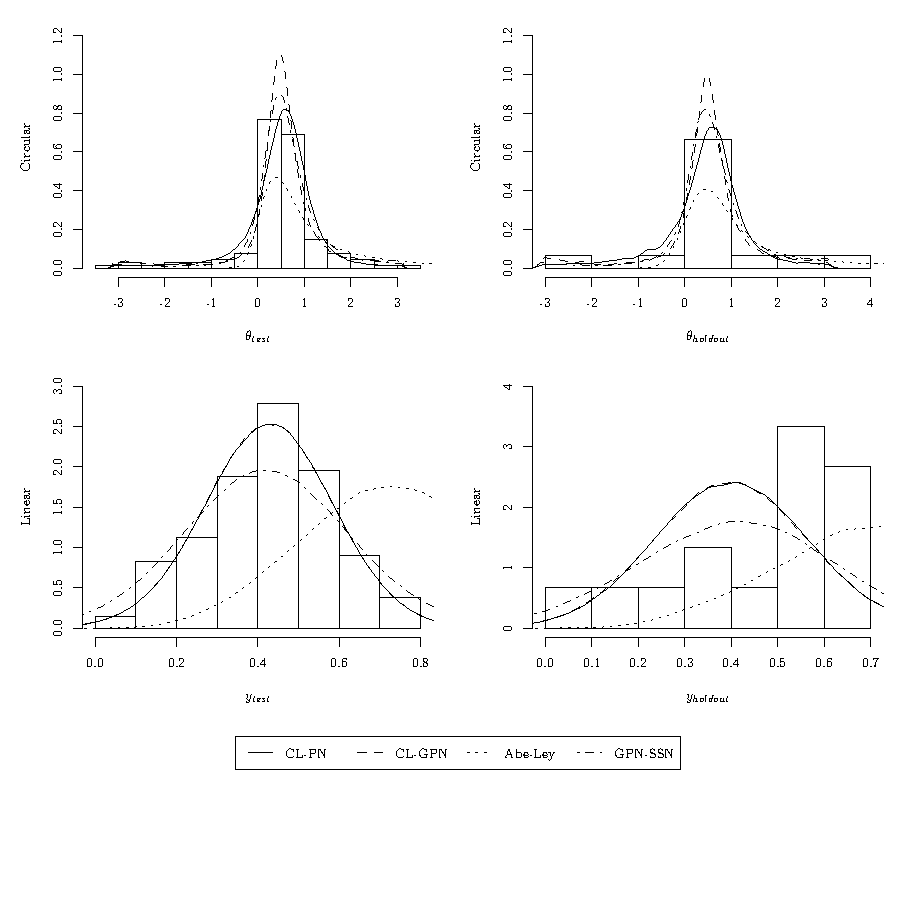
\includegraphics[width = 0.8\textwidth]{preddist.pdf}
\caption{Histograms of $\boldsymbol{y}$ and $\boldsymbol{\theta}$ values of the test and holdout set of the teacher data plotted together with (posterior predictive) density estimates for the modified CL-PN, CL-GPN, Abe-Ley and joint GPN-SSN models.}
\label{preddist}
\end{figure}

\section{Discussion}\label{Discussion}

\begin{itemize}
\item Comment on difficulty of interpreting parameters in GPN model.
\end{itemize}

\newpage
\section*{References}

\hypertarget{refs}{}
\leavevmode\hypertarget{ref-abe2017tractable}{}%
Abe, T., \& Ley, C. (2017). A tractable, parsimonious and flexible model
for cylindrical data, with applications. \emph{Econometrics and
Statistics}, \emph{4}, 91--104.

\leavevmode\hypertarget{ref-chrastil2017rotational}{}%
Chrastil, E. R., \& Warren, W. H. (2017). Rotational error in path
integration: Encoding and execution errors in angle reproduction.
\emph{Experimental Brain Research}, \emph{235}(6), 1885--1897.

\leavevmode\hypertarget{ref-Claessens2016side}{}%
Claessens, L. C. (2016). \emph{Be on my side i'll be on your side :
Teachers' perceptions of teacher--student relationships} (PhD thesis).

\leavevmode\hypertarget{ref-Cremers2018Assessing}{}%
Cremers, J., Mainhard, M. T., \& Klugkist, I. (2018a). Assessing a
bayesian embedding approach to circular regression models.
\emph{Methodology}.

\leavevmode\hypertarget{ref-CremersMulderKlugkist2017}{}%
Cremers, J., Mulder, K. T., \& Klugkist, I. (2018b). Circular
interpretation of regression coefficients. \emph{British Journal of
Mathematical and Statistical Psychology}, \emph{71}(1), 75--95.
doi:\href{https://doi.org/10.1111/bmsp.12108}{10.1111/bmsp.12108}

\leavevmode\hypertarget{ref-garcia2014test}{}%
García-Portugués, E., Barros, A. M., Crujeiras, R. M.,
González-Manteiga, W., \& Pereira, J. (2014). A test for
directional-linear independence, with applications to wildfire
orientation and size. \emph{Stochastic Environmental Research and Risk
Assessment}, \emph{28}(5), 1261--1275.

\leavevmode\hypertarget{ref-garcia2013exploring}{}%
García-Portugués, E., Crujeiras, R. M., \& González-Manteiga, W. (2013).
Exploring wind direction and so2 concentration by circular--linear
density estimation. \emph{Stochastic Environmental Research and Risk
Assessment}, \emph{27}(5), 1055--1067.

\leavevmode\hypertarget{ref-BDA}{}%
Gelman, A., Carlin, J., Stern, H., Dunson, D., Vehtari, A., \& Rubin, D.
(2014). \emph{Bayesian data analysis} (3rd ed.). Boca Raton, FL: Chapman
\& Hall/CRC.

\leavevmode\hypertarget{ref-gneiting2007strictly}{}%
Gneiting, T., \& Raftery, A. E. (2007). Strictly proper scoring rules,
prediction, and estimation. \emph{Journal of the American Statistical
Association}, \emph{102}(477), 359--378.

\leavevmode\hypertarget{ref-gurtman2009exploring}{}%
Gurtman, M. B. (2009). Exploring personality with the interpersonal
circumplex. \emph{Social and Personality Psychology Compass},
\emph{3}(4), 601--619.
doi:\href{https://doi.org/10.1111/j.1751-9004.2009.00172.x}{10.1111/j.1751-9004.2009.00172.x}

\leavevmode\hypertarget{ref-hernandez2016general}{}%
Hernandez-Stumpfhauser, D., Breidt, F. J., \& Woerd, M. J. van der.
(2016). The general projected normal distribution of arbitrary
dimension: Modeling and bayesian inference. \emph{Bayesian Analysis},
\emph{12}(1).
doi:\href{https://doi.org/10.1214/15-BA989}{10.1214/15-BA989}

\leavevmode\hypertarget{ref-horowitz2010handbook}{}%
Horowitz, L. M., \& Strack, S. (2011). \emph{Handbook of interpersonal
psychology: Theory, research, assessment, and therapeutic
interventions}. Hoboken, NJ: John Wiley \& Sons.

\leavevmode\hypertarget{ref-jammalamadaka2001topics}{}%
Jammalamadaka, S. R., \& Sengupta, A. (2001). \emph{Topics in circular
statistics} (Vol. 5). World Scientific.

\leavevmode\hypertarget{ref-johnson1978some}{}%
Johnson, R. A., \& Wehrly, T. E. (1978). Some angular-linear
distributions and related regression models. \emph{Journal of the
American Statistical Association}, \emph{73}(363), 602--606.

\leavevmode\hypertarget{ref-lagona2015hidden}{}%
Lagona, F., Picone, M., Maruotti, A., \& Cosoli, S. (2015). A hidden
markov approach to the analysis of space--time environmental data with
linear and circular components. \emph{Stochastic Environmental Research
and Risk Assessment}, \emph{29}(2), 397--409.

\leavevmode\hypertarget{ref-ley2017modern}{}%
Ley, C., \& Verdebout, T. (2017). \emph{Modern directional statistics}.
CRC Press.

\leavevmode\hypertarget{ref-mardia2000directional}{}%
Mardia, K. V., \& Jupp, P. E. (2000). \emph{Directional statistics}
(Vol. 494). Chichester, England: Wiley.

\leavevmode\hypertarget{ref-mardia1978model}{}%
Mardia, K., \& Sutton, T. (1978). A model for cylindrical variables with
applications. \emph{Journal of the Royal Statistical Society. Series B
(Methodological)}, 229--233.

\leavevmode\hypertarget{ref-mastrantonio2018joint}{}%
Mastrantonio, G. (2018). The joint projected normal and skew-normal: A
distribution for poly-cylindrical data. \emph{Journal of Multivariate
Analysis}, \emph{165}, 14--26.

\leavevmode\hypertarget{ref-mastrantonio2015bayesian}{}%
Mastrantonio, G., Maruotti, A., \& Jona-Lasinio, G. (2015). Bayesian
hidden markov modelling using circular-linear general projected normal
distribution. \emph{Environmetrics}, \emph{26}(2), 145--158.

\leavevmode\hypertarget{ref-nunez2011bayesian}{}%
Nuñez-Antonio, G., Gutiérrez-Peña, E., \& Escarela, G. (2011). A
Bayesian regression model for circular data based on the projected
normal distribution. \emph{Statistical Modelling}, \emph{11}(3),
185--201.
doi:\href{https://doi.org/10.1177/1471082X1001100301}{10.1177/1471082X1001100301}

\leavevmode\hypertarget{ref-olmos2012extension}{}%
Olmos, N. M., Varela, H., Gómez, H. W., \& Bolfarine, H. (2012). An
extension of the half-normal distribution. \emph{Statistical Papers},
\emph{53}(4), 875--886.

\leavevmode\hypertarget{ref-pennings2017interpersonal}{}%
Pennings, H. J., Brekelmans, M., Sadler, P., Claessens, L. C., Want, A.
C. van der, \& Tartwijk, J. van. (2017). Interpersonal adaptation in
teacher-student interaction. \emph{Learning and Instruction}.

\leavevmode\hypertarget{ref-rayner200935th}{}%
Rayner, K. (2009). The 35th sir frederick bartlett lecture: Eye
movements and attention in reading, scene perception, and visual search.
\emph{Quarterly Journal of Experimental Psychology}, \emph{62}(8),
1457--1506.

\leavevmode\hypertarget{ref-sahu2003new}{}%
Sahu, S. K., Dey, D. K., \& Branco, M. D. (2003). A new class of
multivariate skew distributions with applications to bayesian regression
models. \emph{Canadian Journal of Statistics}, \emph{31}(2), 129--150.

\leavevmode\hypertarget{ref-wang2012directional}{}%
Wang, F., \& Gelfand, A. E. (2013). Directional data analysis under the
general projected normal distribution. \emph{Statistical Methodology},
\emph{10}(1, 1), 113--127.
doi:\href{https://doi.org/10.1016/j.stamet.2012.07.005}{10.1016/j.stamet.2012.07.005}

\leavevmode\hypertarget{ref-wang2015joint}{}%
Wang, F., Gelfand, A. E., \& Jona-Lasinio, G. (2015). Joint
spatio-temporal analysis of a linear and a directional variable:
Space-time modeling of wave heights and wave directions in the adriatic
sea. \emph{Statistica Sinica}, 25--39.

\leavevmode\hypertarget{ref-vanderWant2015role}{}%
Want, A. C. van der. (2015). \emph{Teachers' interpersonal role
identity.} (PhD thesis).

\leavevmode\hypertarget{ref-wubbels2006interpersonal}{}%
Wubbels, T., Brekelmans, M., Brok, P. den, \& Tartwijk, J. van. (2006).
An interpersonal perspective on classroom management in secondary
classrooms in the netherlands. In C. Evertson \& C. S. Weinstein (Eds.),
\emph{Handbook of classroom management: Research, practice, and
contemporary issues} (pp. 1161--1191). Malwah, NJ: Lawrence Erlbaum
Associates.

\newpage
\begin{appendices}
\section{Appendix}\label{Appendix}

In this appendix we outline the MCMC procedures to fit the cylindrical regression models from Section \ref{Models}. R-code for the MCMC sampler and the analysis of the teacher data can be found here: \url{https://github.com/joliencremers/CylindricalComparisonCircumplex}.

\subsection{Bayesian Model and MCMC procedure for the modified CL-PN model}\label{A1}

We use the following algorithm to obtain posterior estimates from the model:

\begin{enumerate}

\item Split the data, with the circular outcome $\boldsymbol{\theta} = \theta_i, \dots, \theta_n$, the linear outcome $\boldsymbol{y} = y_i, \dots, y_n$ where $n$ is the sample size, and the design matrices $\boldsymbol{Z}^k$ and $\boldsymbol{X}$ for the two components of the circular and the linear outcome respectively in a training (90\%) and holdout (10\%) set.

\item Define the prior parameters for the training set. In this paper we use:

\begin{itemize}
\item Prior for $\boldsymbol{\gamma}$: $N_q(\boldsymbol{\mu}_{0}, \boldsymbol{\Lambda}_{0})$, with  $\boldsymbol{\mu}_{0} = (0,0,0,0)^t$ and  $\boldsymbol{\Lambda}_{0} = 10^{-4}\boldsymbol{I}_4$.
\item Prior for $\sigma^2$: $IG(\alpha_{0}, \beta_{0})$, an inverse-gamma prior with $\alpha_{0} = 0.001$ and  $\beta_{0} = 0.001$.
\item Prior for $\boldsymbol{\beta^{k}}$: $N_2(\boldsymbol{\mu}_{0}, \boldsymbol{\Lambda}_{0})$, with $\boldsymbol{\mu}_{0} = (0,0)^t$ and  $\boldsymbol{\Lambda}_{0} = 10^{-4}\boldsymbol{I}_2$ for $k \in I,II$.
\end{itemize}

\item Set starting values $\boldsymbol{\gamma} = (0,0,0,0)^t$, $\sigma^2 = 1$ and $\boldsymbol{\beta^{k}} = (0,0)$ for $k \in I,II$. Also set starting values $r_i = 1$ in the training and holdout set. 

\item Compute the latent bivariate outcome $\boldsymbol{s}_i = (s_i^{I}, s_i^{II})^t$ underlying the circular outcome for the holdout and training dataset as follows:

$$\begin{bmatrix} s^{I}_{i} \\ s^{II}_{i} \end{bmatrix} = \begin{bmatrix} r_i \cos \theta_i \\  r_i\sin \theta_i\end{bmatrix}$$

\item Sample $\boldsymbol{\gamma}$, $\sigma^2$ and $\boldsymbol{\beta^{k}}$ for $k \in I,II$ for the training dataset from their conditional posteriors:

\begin{itemize}
\item Posterior for $\boldsymbol{\gamma}$: $N_q(\boldsymbol{\mu}_n, \sigma^2\boldsymbol{\Lambda}^{-1}_n)$, with $\boldsymbol{\mu}_n = (\boldsymbol{X}^t\boldsymbol{X} + \boldsymbol{\Lambda}_0)^{-1}(\boldsymbol{\Lambda}_0\boldsymbol{\mu}_0 + \boldsymbol{X}^t\boldsymbol{y})$ and $\boldsymbol{\Lambda}_n = (\boldsymbol{X}^t\boldsymbol{X} + \boldsymbol{\Lambda}_0)$.
\item Posterior for $\sigma^2$: $IG(\alpha_{n}, \beta_{n})$, an inverse-gamma posterior with $\alpha_{n} = \alpha_0 + n/2$ and $\beta_{n} = \beta_0 + \frac{1}{2}(\boldsymbol{y}^t\boldsymbol{y} + \boldsymbol{\mu}_{0}^t\boldsymbol{\Lambda}_0\boldsymbol{\mu}_{0} + \boldsymbol{\mu}_{n}^t\boldsymbol{\Lambda}_n\boldsymbol{\mu}_{n})$.
\item Posterior for $\boldsymbol{\beta^{k}}$: $N_2(\boldsymbol{\mu}^k_n, \boldsymbol{\Lambda}^{k}_n)$, with $\boldsymbol{\mu}^k_n = ((\boldsymbol{Z}^k)^t\boldsymbol{Z}^k + \boldsymbol{\Lambda}^k_0)^{-1}(\boldsymbol{\Lambda}^k_0\boldsymbol{\mu}^k_0 + (\boldsymbol{Z}^k)^t\boldsymbol{s}^k)$ and $\boldsymbol{\Lambda}^{k}_n = ((\boldsymbol{Z}^k)^t\boldsymbol{Z}^k + \boldsymbol{\Lambda}^k_0)$.
\end{itemize}

\item Sample new $r_i$ for the training and holdout dataset from the following posterior:

$$f(r_i \mid \theta_i, \boldsymbol{\mu}_i) \propto r_i \exp{(-\frac{1}{2}(r_i)^2 + b_ir_i)}$$ 
where $b_i = \begin{bmatrix} \cos \theta_i \\ \sin \theta_i\end{bmatrix}^t\boldsymbol{\mu}_i$, $\boldsymbol{\mu}_i = \boldsymbol{z_i}\boldsymbol{B}$ and $\boldsymbol{B} = (\boldsymbol{\beta}^{I}, \boldsymbol{\beta}^{II})$. 

We can sample from this posterior using a slice sampling technique (Cremers et al., 2018): 

\begin{itemize}
\item In a slice sampler the joint density for an auxiliary variable $v_{i}$ with $r_{i}$ is:


$$p(r_{i}, v_{i}\mid \theta_{i}, \boldsymbol{\mu}_{i}=\boldsymbol{z}_{i}\boldsymbol{B}) \propto r_{i} \textbf{I}\left(0 < v_i < \exp\left\{ -\frac{1}{2}(r_{i} - b_{i})^2\right\}\right)\textbf{I}(r_i > 0).$$

\noindent The full conditional for $v_{i}$, $p(v_{i} \mid r_{i},\boldsymbol{\mu}_{i}, \theta_{i})$, is:

$$U\left(0, \exp\left\{-\frac{1}{2}(r_{i} -  b _{i})^2\right\}\right)$$

and the full conditional for $r_i$, $p(r_{i} \mid v_{i},\boldsymbol{\mu}_{i}, \theta_{i})$, is proportional to:
$$r_{i} \textbf{I}\left(b_{i} + \max\left\{-b_{i}, -\sqrt{-2\ln v_{i}}\right\} < r_{i} < b_{i} + \sqrt{-2\ln v_{i}}\right).$$

\noindent We thus sample $v_{i}$ from the uniform distribution specified above. Independently we sample a value $m$ from $U(0,1)$. We obtain a new value for $r_{i}$ by computing $ r_{i} = \sqrt{(r_{i_{2}}^{2}-r_{i_{1}}^{2})m + r_{i_{1}}^{2}}$ where $r_{i_{1}}=b_{i} +\max\left\{-b_{i}, -\sqrt{-2\ln v_{i}}\right\}$ and $ r_{i_{2}}= b_{i} + \sqrt{-2\ln v_{i}}$.
\end{itemize}

\item Compute the PLSL for the circular and linear outcome on the holdout set using the estimates of $\boldsymbol{\gamma}$, $\sigma^2$ and $\boldsymbol{\beta^{k}}$ for $k \in I,II$ for the training dataset.

\item Repeat steps 4 to 8 until the sampled parameter estimates have converged.

\end{enumerate}





\newpage
\subsection{Bayesian Model and MCMC procedure for the modified CL-GPN mode}\label{A2}

We use the following algorithm to obtain posterior estimates from the model:

\begin{enumerate}

\item Split the data, with the circular outcome $\boldsymbol{\theta} = \theta_i, \dots, \theta_n$, the linear outcome $\boldsymbol{y} = y_i, \dots, y_n$ where $n$ is the sample size, and the design matrices $\boldsymbol{Z}^k$ and $\boldsymbol{X}$ for the two components of the circular and the linear outcome respectively in a training (90\%) and holdout (10\%) set.

\item Define the prior parameters for the training set. In this paper we use:

\begin{itemize}
\item Prior for $\boldsymbol{\gamma}$: $N_q(\boldsymbol{\mu}_{0}, \boldsymbol{\Lambda}_{0})$, with $\boldsymbol{\mu}_{0} = (0,0,0,0)^t$ and $\boldsymbol{\Lambda}_{0} = 10^{-4}\boldsymbol{I}_4$.
\item Prior for $\sigma^2$: $IG(\alpha_{0}, \beta_{0})$, an inverse-gamma prior with $\alpha_{0} = 0.001$ and $\beta_{0} = 0.001$.
\item Prior for $\boldsymbol{\beta}_{j}$: $N_2(\boldsymbol{\mu}_{0}, \boldsymbol{\Lambda}_0)$, with $\boldsymbol{\mu}_{0} = (0,0)^t$ and  $\boldsymbol{\Sigma}_{0} = 10^{5}\boldsymbol{I}_2$ for $j \in 1, \dots, p$ where $p$ is the number of covariates in $\boldsymbol{Z}$.
\item Prior for $\rho$: $N(\mu_0, \sigma^2)$, with $\mu_0 = 0$ and $\sigma^2 = 10^{4}$.
\item Prior for $\tau$: $IG(\alpha_{0}, \beta_{0})$, an inverse gamma prior with $\alpha_{0} = 0.01$ and $\beta_{0} = 0.01$.
\end{itemize}


\item Set starting values $\boldsymbol{\gamma} = (0,0,0,0)^t$, $\sigma^2 = 1$, $\boldsymbol{\beta}_j = (0,0)^t$, $\rho = 0$, $\tau = 1$ and $\boldsymbol{\Sigma} = \begin{bmatrix} \tau^2 + \rho^2 & \rho\\ \rho & 1 \end{bmatrix}$. Also set starting values $r_i = 1$ in the training and holdout set. 

\item Compute the latent bivariate outcome $\boldsymbol{s}_i = (s_i^{I}, s_i^{II})^t$ underlying the circular outcome for the holdout and training dataset as follows:

$$\begin{bmatrix} s^{I}_{i} \\ s^{II}_{i} \end{bmatrix} = \begin{bmatrix} r_i \cos \theta_i \\  r_i\sin \theta_i\end{bmatrix}$$

\item Sample $\boldsymbol{\gamma}$, $\sigma^2$, $\boldsymbol{\beta}_j$, $\rho$ and $\tau$ for the training dataset from their conditional posteriors:

\begin{itemize}
\item Posterior for $\boldsymbol{\gamma}$: $N_q(\boldsymbol{\mu}_n, \sigma^2\boldsymbol{\Lambda}^{-1}_n)$, with $\boldsymbol{\mu}_n = (\boldsymbol{X}^t\boldsymbol{X} + \boldsymbol{\Lambda}_0)^{-1}(\boldsymbol{\Lambda}_0\boldsymbol{\mu}_0 + \boldsymbol{X}^t\boldsymbol{y})$ and $\boldsymbol{\Lambda}_n = (\boldsymbol{X}^t\boldsymbol{X} + \boldsymbol{\Lambda}_0)$.
\item Posterior for $\sigma^2$: $IG(\alpha_{n}, \beta_{n})$, an inverse-gamma posterior where $\alpha_{n} = \alpha_0 + n/2$ and $\beta_{n} = \beta_0 + 0.5(\boldsymbol{y}^t\boldsymbol{y} + \boldsymbol{\mu}_{0}^t\boldsymbol{\Lambda}_0\boldsymbol{\mu}_{0} + \boldsymbol{\mu}_{n}^t\boldsymbol{\Lambda}_n\boldsymbol{\mu}_{n})$.
\item Posterior for $\boldsymbol{\beta}_j$: $N_2(\boldsymbol{\mu}_{j_{n}}, \boldsymbol{\Sigma}_{j_{n}})$, with $\boldsymbol{\mu}_{j_{n}} = \boldsymbol{\Sigma}_{j_{n}}\boldsymbol{\Sigma}^{-1}\Bigg(-\sum_{i=1}^{n}z_{i,j-1}\sum_{l\neq j}z_{i,l-1}\boldsymbol{\beta}_l + \sum_{i=1}^{n}z_{i,j-1}r_i\begin{bmatrix} \cos \theta_i \\ \sin \theta_i\end{bmatrix}\Bigg)$ and  $\boldsymbol{\Sigma}_{j_{n}} = \Big(\sum_{i=1}^{n}z_{i,j-1}^2\boldsymbol{\Sigma}^{-1}+\boldsymbol{\Lambda}_0\Big)^{-1}$ for $j \in 1, \dots, p$ where p is the number of covariates in $\boldsymbol{Z}$.
\item Posterior for $\rho$: $N(\mu_n, \sigma^2_n)$, with $\mu_n = \frac{\tau^{-2} \sum_{i=1}^{n}(s^{I}_{i} - \mu_i^{I})(s^{II}_{i} - \mu_i^{II}) + \mu_0\sigma_0^{-2}}{\tau^{-2}\sum_{i=1}^{n}(s^{II}_{i} - \mu^{II})^2 + \sigma_0^{-2}}$ and $\sigma_n^2 = \frac{1}{\tau^{-2}\sum_{i=1}^{n}(s^{II}_{i} - \mu^{II})^2 + \sigma_0^{-2}}$ where $\mu_i^{I} = \boldsymbol{z}_i\boldsymbol{\beta}^{I}$ and $\mu_i^{II} = \boldsymbol{z}_i\boldsymbol{\beta}^{II}$.
\item Posterior for $\tau$: $IG(\alpha_n, \beta_n)$, an inverse-gamma posterior with $\alpha_n = \frac{n}{2} + \alpha_0$ and $\beta_n = \sum\limits_{i = 1}^{n}(s^{I}_{i} - \{\mu_i^{II} + \rho(s^{II}_{i} - \mu^{II})\})^2 + \beta_0$
\end{itemize}

\item Sample new $r_i$ for the training and holdout dataset from the following posterior:

$$f(r_i \mid \theta_i, \boldsymbol{\mu}_i) \propto r_i \exp{\left\{-0.5A_i\bigg(r_i-\frac{B_i}{A_i}\bigg)^2\right\}}$$ 
where $B_i = \begin{bmatrix} \cos \theta_i \\ \sin \theta_i\end{bmatrix}^t\boldsymbol{\Sigma}^{-1}\boldsymbol{\mu}_i$, $\boldsymbol{\mu}_i = \boldsymbol{z_i}\boldsymbol{B}$, $\boldsymbol{B} = (\boldsymbol{\beta}^{I}, \boldsymbol{\beta}^{II})$ and $A_i = \begin{bmatrix} \cos \theta_i \\ \sin \theta_i\end{bmatrix}^t\boldsymbol{\Sigma}^{-1}\begin{bmatrix} \cos \theta_i \\ \sin \theta_i\end{bmatrix}$.

We can sample from this posterior using a slice sampling technique (Hernandez-Stumpfhauser et.al. 2018):

\begin{itemize}
\item In a slice sampler the joint density for an auxiliary variable $v_{i}$ with $r_{i}$ is:

$$p(r_{i}, v_{i}\mid \theta_{i}, \boldsymbol{\mu}_{i}=\boldsymbol{z}_{i}\boldsymbol{B}^{t}) \propto r_{i} \textbf{I}\bigg(0 < v_i < \exp\left\{ -.5 A_i(r_{i} - \frac{B_i}{A_i})^2\right\}\bigg)\textbf{I}(r_i > 0)$$

\item The full conditional for $v_{i}$, $p(v_{i} \mid r_{i},\boldsymbol{\mu}_{i}, \boldsymbol{\Sigma}, \theta_{i})$, is:

$$U\Bigg(0, \exp\left\{-.5A_i\bigg(r_i -  \frac{B_{i}}{A_i}\bigg)^2\right\}\Bigg)$$
and the full conditional for $r_i$, $p(r_{i} \mid v_{i},\boldsymbol{\mu}_{i}, \boldsymbol{\Sigma}, \theta_{i})$, is proportional to:
$$r_{i} \textbf{I}\left(\frac{B_i}{A_i} + \max\left\{-\frac{B_i}{A_i}, -\sqrt{\frac{-2\ln v_{i}}{A_i}}\right\} < r_{i} < \frac{B_i}{A_i} + \sqrt{\frac{-2\ln v_{i}}{A_i}}\right)$$
\item We thus sample $v_{i}$ from the uniform distribution specified above. Independently we sample a value $m$ from $U(0,1)$. We obtain a new value for $r_{i}$ by computing $r_{i} = \sqrt{(r_{i_{2}}^{2}-r_{i_{1}}^{2})m + r_{i_{1}}^{2}}$ where $r_{i_{1}}=\frac{B_i}{A_i} +\max\left\{-\frac{B_i}{A_i}, -\sqrt{\frac{-2\ln v_{i}}{A_i}}\right\}$ and $ r_{i_{2}}= \frac{B_i}{A_i} + \sqrt{\frac{-2\ln v_{i}}{A_i}}$.

\end{itemize}

\item Compute the PLSL for the circular and linear outcome on the holdoutset using the estimates of $\boldsymbol{\gamma}$, $\sigma^2$, $\boldsymbol{\beta^{k}}$, $\rho$ and $\tau$ for the training dataset. Use the density $f(\theta, r \mid \boldsymbol{\mu}, \boldsymbol{\Sigma})$ for the circular outcome.

\item Repeat steps 4 to 8 until the sampled parameter estimates have converged.

\end{enumerate}





\newpage
\subsection{Bayesian Model and MCMC procedure multivariate GPN model}\label{A3}

\begin{enumerate}
\item Split the data, with the circular outcome $\boldsymbol{\theta} = \theta_i, \dots, \theta_n$, the linear outcome $\boldsymbol{y} = y_i, \dots, y_n$ where $n$ is the sample size, and the design matrix $\boldsymbol{X}$ in a training (90\%) and holdout (10\%) set. Note that in this paper we have only one circular outcome and one linear outcome and the MCMC procedure outlined here is specified for this situation. It can however be generalized to a situation with multiple circular and linear outcomes without too much effort. 

\item Define the prior parameters for the training set. Note that in this paper we have only one circular outcome and one linear outcome, so $p = 1$ and $q = 1$. In this paper we use the following priors:

\begin{itemize}
\item Prior for $\boldsymbol{\Sigma}$: $IW(\boldsymbol{\Psi}_0, \nu_0)$, an inverse-Wishart with $\boldsymbol{\Psi}_0 = 10^{-4}\boldsymbol{I}_{2p + q}$ and $\nu_0 = 1$.   
\item Prior for $\boldsymbol{\beta}$: $MN(\boldsymbol{\beta}_0, \boldsymbol{\Sigma}_0  \otimes \boldsymbol{\kappa}_0)$, where $\boldsymbol{\beta}$ is a vectorized $\boldsymbol{B}$, the matrix with regression coefficients, $\boldsymbol{\beta}_0 = \boldsymbol{0}_{k(2p + q)}$, $\boldsymbol{B}_0 = \boldsymbol{0}_{k \times (2p + q)}$ and $\boldsymbol{\kappa}_0 = 10^{-4}\boldsymbol{I}_k$.
\item Prior for $\lambda$: $N(\gamma_0, \omega_0)$, with $\gamma_0 = 0$ and $\omega_0 = 10000$.
\end{itemize}

\item Set starting values $\boldsymbol{\beta} = (0,0,0,0,0,0)^t$, $\boldsymbol{\Sigma} = \boldsymbol{I}_3$ and $\lambda = 0$. Also set starting values $r_i = 1$ and $d_i = 1$ in the training and holdout set. 

\item Compute the latent bivariate outcome $\boldsymbol{s}_i = (s_i^{I}, s_i^{II})^t$ underlying the circular outcome for the holdout and training dataset as follows:

$$\begin{bmatrix} s^{I}_{i} \\ s^{II}_{i} \end{bmatrix} = \begin{bmatrix} r_i \cos \theta_i \\  r_i\sin \theta_i\end{bmatrix}$$
\item Compute the latent outcomes $\tilde{y}_i$ underlying the linear outcome for the holdout and training dataset as follows:

$$\tilde{y}_i = \lambda d_i $$

\item Compute $\boldsymbol{\eta}_i$ defined as follows for each individual i:

$$\boldsymbol{\eta}_i = (\boldsymbol{s}_i,y_i)^t - (\boldsymbol{0}_{2p}, \lambda d_i)$$

\item Sample $\boldsymbol{B}$, $\boldsymbol{\Sigma}$ and $\lambda$ for the training dataset from their conditional posteriors:

\begin{itemize}
\item Posterior for $\boldsymbol{B}$: $MN(\boldsymbol{B}_n, \boldsymbol{\kappa}_n, \boldsymbol{\Sigma}_n)$, with $\boldsymbol{B}_n = \boldsymbol{\kappa}_n^{-1}\boldsymbol{X}^t\boldsymbol{\eta} + \boldsymbol{\kappa}_0\boldsymbol{B}_0$ and $\boldsymbol{\kappa}_n = \boldsymbol{X}^t\boldsymbol{X} + \boldsymbol{\kappa}_0$.
\item Posterior for $\Sigma$: $IW(\boldsymbol{\Psi}_n, \nu_n)$, an inverse-Wishart with $\boldsymbol{\Psi}_n = \boldsymbol{\Psi}_0 + (\boldsymbol{\eta} - \boldsymbol{X}^t\boldsymbol{B})^t(\boldsymbol{\eta} - \boldsymbol{X}^t\boldsymbol{B}) + (\boldsymbol{B} - \boldsymbol{B}_0)^t\boldsymbol{\kappa}_0(\boldsymbol{B} - \boldsymbol{B}_0)$ and $\nu_n = \nu_0 + n$
\item Posterior for $\lambda$: $N(\gamma_n, \omega_n)$, with $\omega_n = \big(\sum_{i = 1}^{n}d_i^2\boldsymbol{\Sigma}_{y|s}^{-1} + \omega_0^{-1}\big)^{-1}$ and $\gamma_n = \omega_n \big(\sum_{i = 1}^{n}d_i\boldsymbol{\Sigma}_{y|s}^{-1}(y_i - \boldsymbol{\mu}_{y_i|s_i}) + \omega_0^{-1}\gamma_0 \big)$
\end{itemize}

\item Sample new $d_i$ for the training and holdout dataset from the following posterior:

$$f(d_i) \propto \phi_q(y_i|\boldsymbol{\mu}_{y_i|s_i} + \lambda d_i, \boldsymbol{\Sigma}_{y|s})\phi_q(d_i|0, 1),$$

where $\boldsymbol{\mu}_{y_i|s_i} = \boldsymbol{x}_i\boldsymbol{B}_{y_i|s_i}$. We can see $d_i$ as a positive regressor with $\lambda$ as covariate and $\phi_q(d_i|0, 1)$ as prior (Mastrantonio, 2018). The full conditional is then a q-dimensional truncated normal with support $\mathbb{R}^{+}$ as follows:

$$N_q(\boldsymbol{M}_{d_i}, \boldsymbol{V}_q),$$ \\where $\boldsymbol{V}_q = \big(\lambda^2\boldsymbol{\Sigma}_{y|s}^{-1} + 1\big)$ and $\boldsymbol{M}_{d_i} = \boldsymbol{V}_d\lambda\boldsymbol{\Sigma}_{y|s}^{-1}\big(y_i - \boldsymbol{\mu}_{y_i, s_i}\big)$.

\item Sample new $r_i$ for the training and holdout dataset from the following posterior:

$$f(r_i \mid \theta_i, \boldsymbol{\mu}_i) \propto r_i \exp{\left\{-0.5A_i\bigg(r_i-\frac{B_i}{A_i}\bigg)^2\right\}}$$ 
where $B_i = \begin{bmatrix} \cos \theta_i \\ \sin \theta_i\end{bmatrix}^t\boldsymbol{\Sigma}_{s_i|y_i}^{-1}\boldsymbol{\mu}_{s_i|y_i}$, $\boldsymbol{\mu}_{s_i|y_i} = \boldsymbol{x}_i\boldsymbol{B}_{s_i|y_i}$ and $A_i = \begin{bmatrix} \cos \theta_i \\ \sin \theta_i\end{bmatrix}^t\boldsymbol{\Sigma}_{s_i| y_i}^{-1}\begin{bmatrix} \cos \theta_i \\ \sin \theta_i\end{bmatrix}$. The parameters $\boldsymbol{\mu}_{s_i|y_i}$ and $\boldsymbol{\Sigma}_{s_i| y_i}$ are the conditional mean and covariance matrix of $\boldsymbol{s}_i$ assuming that $(\boldsymbol{s}_i, y_i)^t \sim N_{2p+q}(\boldsymbol{\mu} + (\boldsymbol{0}_{2p}, \lambda d_i)^t, \boldsymbol{\Sigma})$.

Because in this paper $\boldsymbol{\theta}$ originates from a bivariate variable that is known we can simply define the $r_i$ as the euclidean norm of the bivariate datapoints. However, for didactic purposes continue with the explanation of the sampling procedure. We
can sample from posterior for $r_i$ using a slice sampling technique (Hernandez-Stumpfhauser et.al. 2018):

\begin{itemize}
\item In a slice sampler the joint density for an auxiliary variable $v_{i}$ with $r_{i}$ is:

$$p(r_{i}, v_{i}\mid \theta_{i}, \boldsymbol{\mu}_{i}=\boldsymbol{x}_{i}\boldsymbol{B}^{t}) \propto r_{i} \textbf{I}\bigg(0 < v_i < \exp\left\{ -.5 A_i(r_{i} - \frac{B_i}{A_i})^2\right\}\bigg)\textbf{I}(r_i > 0)$$

\item The full conditionals for $v_{i}$, $p(v_{i} \mid r_{i},\boldsymbol{\mu}_{i}, \boldsymbol{\Sigma}, \theta_{i})$, is:

$$U\Bigg(0, \exp\left\{-.5A_i\bigg(r_i -  \frac{B_{i}}{A_i}\bigg)^2\right\}\Bigg)$$
and the full conditional for $r_i$, $p(r_{i} \mid v_{i},\boldsymbol{\mu}_{i}, \boldsymbol{\Sigma}, \theta_{i})$ , is proportional to :
$$r_{i} \textbf{I}\left(\frac{B_i}{A_i} + \max\left\{-\frac{B_i}{A_i}, -\sqrt{\frac{-2\ln v_{i}}{A_i}}\right\} < r_{i} < \frac{B_i}{A_i} + \sqrt{\frac{-2\ln v_{i}}{A_i}}\right)$$
\item We thus sample $v_{i}$ from the uniform distribution specified above. Independently we sample a value $m$ from $U(0,1)$. We obtain a new value for $r_{i}$ by computing $r_{i} = \sqrt{(r_{i_{2}}^{2}-r_{i_{1}}^{2})m + r_{i_{1}}^{2}}$ where $r_{i_{1}}=\frac{B_i}{A_i} +\max\left\{-\frac{B_i}{A_i}, -\sqrt{\frac{-2\ln v_{i}}{A_i}}\right\}$ and $ r_{i_{2}}= \frac{B_i}{A_i} + \sqrt{\frac{-2\ln v_{i}}{A_i}}$.

\end{itemize}

\item Compute the PLSL for the circular and linear outcome on the holdoutset using the estimates of $\boldsymbol{B}$, $\boldsymbol{\Sigma}$ and $\lambda$ for the training dataset.

\item Repeat steps 4 to 10 until the sampled parameter estimates have converged.

\item In the MCMC sampler we have estimated an unconstrained $\boldsymbol{\Sigma}$. However, for identification of the model we need to apply the following constraint to both $\boldsymbol{\Sigma}$ and $\boldsymbol{\mu}$:

$$\boldsymbol{C} = \begin{bmatrix} \boldsymbol{C}_w & \boldsymbol{0}_{2p \times q} \\ \boldsymbol{0}_{2p \times q}^t & \boldsymbol{I}_q \end{bmatrix}$$
where $\boldsymbol{C}_w$ is a $2p \times 2p$ diagonal matrix with every $(2(j-1) + k)^{th}$ entry $> 0$ where $k \in 1, 2$ and $k = 1, \dots, p$ (Mastrantonio, 2018). The estimates $\boldsymbol{\Sigma}$ and $\boldsymbol{\mu}$ can then be related to their constrained versions, $\tilde{\boldsymbol{\Sigma}}$ and $\tilde{\boldsymbol{\mu}}$ as follows:

$$\boldsymbol{\mu} = \boldsymbol{C}\tilde{\boldsymbol{\mu}}$$
$$\boldsymbol{\Sigma} = \boldsymbol{C}\tilde{\boldsymbol{\Sigma}}\boldsymbol{C}.$$

\end{enumerate}

\end{appendices}


\end{document}
